\section{Auswertung}
\label{sec:Auswertung}

\subsection{Bestimmung der Relaxationszeit $T_{2}$ mit der Meiboom-Gill-Methode}
\label{subsec:T2}

Um die Relaxationszeit $T_{2}$ zu bestimmen, werden die Signale, der mit dem Oszilloskop aufgenommenen
Burst-Sequenz der Meiboom-Gill Methode(siehe Abbildung \ref{fig:meiboomgill} und \ref{fig:t2_gesamt}) gegen die Zeit aufgetragen.
Um die $50$ Echoamplituden zu finden, werden ganzzahlige Vielfache von $\tau = \SI{20}{\milli\second}$ multipliziert mit $4$
auf die Zeit, bei der die höchste Spannung gemessen wird, addiert und der jeweils nächstgelegene Messwert innerhalb eines beschränkten Intervalls ausgewählt.
In Tabelle \ref{tab:t2_fitwerte}
sind die auf diese Weise gefundenen Echos angegeben.
Anschließend wird für den in Gleichung \eqref{eqn:11} gegebenen Zusammenhang unter \textit{Python3} mit Hilfe der Funktion \textit{curvefit} aus
dem Paket \textit{Scipy} eine Regression der als Echos identifizierten Messwerte durchgeführt.\\
Dabei ergeben sich für den Startwert $U_{0}$ und Relaxationszeit $T_{2}$ die folgenden Werte
\begin{align*}
  U_{0} &= \SI{0.50+-0.03}{\volt} \\
  T_{2} &= \SI{ 1.04+-0.11}{\second} \, .
\end{align*}
In Abbildung \ref{fig:t2_plot} sind die verwendeten Messwerte, sowie der Graph der zugehörigen Regression
gezeigt.\\


\begin{figure}[hhh]
  \centering
  \includegraphics{build/t_u_plot2_extrem.pdf}
  \caption{Verwendete Messwerte(Signal logarithmiert) für $T_{2}$ Messung mit Meiboom-Gill-Methode, sowie zugehörige Regression.}
  \label{fig:t2_plot_gesamt}
\end{figure}


\begin{figure}[hhh]
  \centering
  \includegraphics{build/t_u_plot2.pdf}
  \caption{Aufgenommene Messwerte für $T_{2}$ Messung mit Meiboom-Gill-Methode.}
  \label{fig:t2_plot}
\end{figure}


\begin{figure}[hhh]
  \centering
  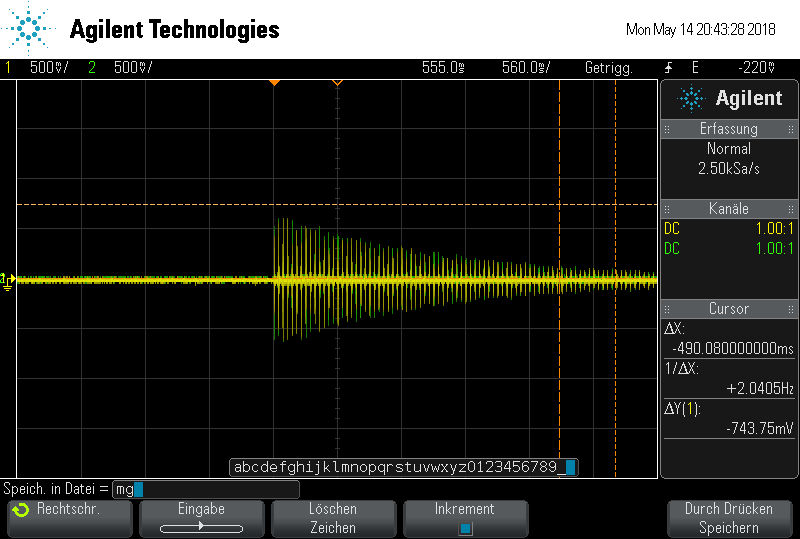
\includegraphics[width=\textwidth]{mg.png}
  \caption{Messwerte für $T_{2}$ Messung mit Meiboom-Gill-Methode(Bild am Oszilloskop).}
  \label{fig:meiboomgill}
\end{figure}

Der Literaturwert\cite{litwerte} für die Relaxationszeit $T_{2}$ von bidestilliertem Wasser
beträgt
\begin{align*}
  T_{2}^\text{lit.} = \SI{1.52+-0.093}{\second},
\end{align*}
sodass sich eine relative Abweichung $f$ des experimentell bestimmten Werts
von
\begin{align*}
  f = \frac{T_{2} - T_{2}^\text{lit.}}{T_{2}^\text{lit.}} = \SI{32+-8}{\percent}
\end{align*}
ergibt.


\begin{table}
  \centering
  \caption{Gefundene Echos für die Bestimmung der Relaxationszeit $T_{2}$.}
  \label{tab:t2_fitwerte}
  \begin{tabular}{c c}
  \toprule
  $t \text{ in } \si{\milli\second}$ & $U \text{ in } \si{\milli\volt}$\\
  \midrule
  0.0	&	561.56   \\ 
81.2	&	461.06   \\ 
162.4	&	320.35   \\ 
238.0	&	219.85   \\ 
319.2	&	420.85   \\ 
400.4	&	320.35   \\ 
476.0	&	79.15   \\ 
560.0	&	239.95   \\ 
641.2	&	159.55   \\ 
722.4	&	219.85   \\ 
798.0	&	119.35   \\ 
879.2	&	280.15   \\ 
963.2	&	79.15   \\ 
1041.6	&	139.45   \\ 
1120.0	&	280.15   \\ 
1201.2	&	38.94   \\ 
1282.4	&	139.45   \\ 
1358.0	&	119.35   \\ 
1439.2	&	199.75   \\ 
1523.2	&	79.15   \\ 
1598.8	&	100.50   \\ 
1677.2	&	59.04   \\ 
1761.2	&	119.35   \\ 
1842.4	&	99.25   \\ 
1918.0	&	79.15   \\ 
1999.2	&	119.35   \\ 
2080.4	&	79.15   \\ 
2161.6	&	59.04   \\ 
2220.4	&	0.00   \\ 
2321.2	&	79.15   \\ 
2396.8	&	38.94   \\ 
2478.0	&	18.84   \\ 
2559.2	&	119.35   \\ 
2643.2	&	38.94   \\ 
2716.0	&	18.84   \\ 
2797.2	&	38.94   \\ 
2881.2	&	79.15   \\ 
2962.4	&	38.94   \\ 
3038.0	&	38.94   \\ 
3119.2	&	38.94   \\ 
3200.4	&	79.15   \\ 
3262.0	&	0.00   \\ 
3343.2	&	0.00   \\ 
3441.2	&	38.94   \\ 
3508.4	&	0.00   \\ 
3598.0	&	20.10   \\ 
3679.2	&	38.94   \\ 
3760.4	&	18.84   \\ 
3827.6	&	0.00   \\ 
3900.4	&	0.00   \\ 
3981.6	&	0.00   \\ 

  \bottomrule
  \end{tabular}
\end{table}


\FloatBarrier
\subsubsection{Bestimmung des Diffusionskoeffizienten mit der Spin-Echo-Methode}
\label{subsec:D}
Der Diffusionskonstante wird aus den in Tabelle \ref{tab:diffusion} angegebenen
Messwerten bestimmt.
Dazu wird eine Regression der Werte für den in Gleichung \eqref{eqn:32} gegebenen Zusammenhang mit
\textit{curvefit} durchgeführt.
Als Fitparameter werden der Vorfaktor $a$ sowie die Diffusionskonstante gewählt. Für $T_{2}$ wird der in Abschnitt
\ref{subsubsec:T2} bestimmte Wert verwendet. Der Gradient $G$ wird aus dem Zusammenhang
\begin{align}
  \label{eqn:gradient}
  G = \frac{8.8}{d \, \gamma \, t_{\frac{1}{2}}}
\end{align}
gewonnen. Dabei bezeichnet $d$ den Probendurchmesser, von $\SI{4.4}{\milli\meter}$, \gamma das gyromagnetische Verhältnis
von Protonen in Wasser und $t_{\frac{1}{2}}$ die Halbwertszeit.
Wird der Ausdruck \eqref{eqn:gradient} in Gleichung \eqref{eqn:32} eingesetzt, ist leicht zu erkennen, dass $\gamma$ wegfällt und nur noch $d$ und $t_{\frac{1}{2}}$ eingesetzt werden müssen.
Die Halbwertszeit wird anhand der Messwerte abgeschätzt, indem die Zeit gewählt wird, deren zugehöriges Signal am ehesten
gleich der Hälfte des maximalen Signals ist.
Da in Gleichung \eqref{eqn:32} die Zeit $t$ verwendet wird, allerdings $\tau$ gemessen wurde, müssen
die gemessenen Werte für die Zeit noch gemäß
\begin{align}
  t = 2 \tau
\end{align}
umgerechnet werden.
Für die Halbwertsbreite ergibt sich grob
\begin{align*}
  t_{\frac{1}{2}} = \SI{0.05}{\second}.
\end{align*}
In Abbildung \ref{fig:diffusion} sind die Messwerte, sowie der Graph der Regression dargestellt.\\
Als Regressionsparameter ergeben sich
\begin{align*}
  a &= \SI{0.7539+-0.0061}{\volt}\\
  D &= \SI{3.8325+-0.1131 e-5}{\meter\squared\per\second} \, .
\end{align*}

\begin{table}
  \centering
  \caption{Verwendete Messwerte für die Bestimmung der Diffusionskonstanten.}
  \label{tab:diffusion}
  \begin{tabular}{c c}
  \toprule
  $t \text{ in } \si{\milli\second}$ & $U \text{ in } \si{\milli\volt}$\\
  \midrule
  0.0	&	793.75   \\ 
5.0	&	750.00   \\ 
10.0	&	737.50   \\ 
15.0	&	718.75   \\ 
20.0	&	700.00   \\ 
25.0	&	675.00   \\ 
30.0	&	634.75   \\ 
35.0	&	593.75   \\ 
40.0	&	500.00   \\ 
45.0	&	443.75   \\ 
50.0	&	387.50   \\ 
55.0	&	306.25   \\ 
60.0	&	243.75   \\ 
65.0	&	181.25   \\ 

  \bottomrule
  \end{tabular}
\end{table}


\begin{figure}[hhh]
  \centering
  \includegraphics{build/t_u_plotdiff.pdf}
  \caption{Messwerte für die Bestimmung des Diffusionskoeffizienten, sowie zugehörige Regression.}
  \label{fig:diffusion}
\end{figure}

\FloatBarrier
\subsubsection{Bestimmung der Viskosität}
\label{subsubsec:viskositaet}
Die Viskosität von Wasser wird mit Hilfe eines Viskosimeters bestimmt.
Am Viskosimeter werden zwei Zeiten gemessen
\begin{align*}
  t_{1}^\text{visk.} &= \SI{723.5+-2}{\second}\\
  t_{2}^\text{visk.} &= \SI{720.3+-2}{\second}\, .
\end{align*}
Es wird mit dem Mittelwert der beiden Zeiten
\begin{align*}
  t^\text{visk.} &= \SI{721.9+-1.4}{\second}
\end{align*}
gerechnet.\\
Um aus der gemessenen Zeit die Viskosität zu bestimmen wird der Zusammenhang\eqref{eqn:viskositaet}
\begin{align}
  \eta = a \left(t - \delta \right)
\end{align}
verwendet. Dabei bezeichnet $a$ eine Apparaturkonstante die mit $a = \SI{1.024e-9}{}$ angegeben wird und $\delta$
eine Apparaturkonstante die mit $\delta = \SI{0.8562+-0.0014}{}$ angegeben wird.
Für die Viskosität ergibt sich auf diese Weise
\begin{align*}
  \eta = \SI{0.7364+-0.0014 e-3}{} \, .
\end{align*}

% weglassen?
Der Literaturwert\cite{lig_v} für die Viskosität ist
\begin{align*}
  \eta^\text{lit.} = \SI{}{} \, ,
\end{align*}
sodass die relative Abweichung $f$ des experimentell bestimmten Werts
vom Theoriewert
\begin{align*}
  f = \frac{\eta - \eta^\text{lit.}}{\eta^\text{lit.}} = \SI{}{\percent}
\end{align*}


\FloatBarrier
\subsubsection{Bestimmung des Molekülradius}
\label{subsubsec:molekuelradius}
Mit bekanntem Diffusionskoeffizienten $D$ und Viskosität $\eta$ kann gemäß
der Stokesschen Formel folgender Zusammenhang für den Molekülradius $R$ hergeleitet werden
\begin{align}
  \label{eqn:stokes}
  R = \frac{k_\text{B} \, T}{6 \pi \, \eta \, D} \, .
\end{align}
Mit den vorher bestimmten Werten ergibt sich für den Molekülradius
\begin{align*}
  R = \SI{7.74+-0.23}{\femto\meter} \, .
\end{align*}
Dieser Wert soll nun verglichen werden, mit dem Molekülradius, der ermittelt werden kann, indem angenommen wird, dass sich
Kugelförmige Wassermoleküle in einer hexagonal dichtesten Packung anordnen.
Für diese Annahme ergibt sich ein Radius von
\begin{align*}
  R = \sqrt{\frac{m}{4\sqrt{2} \, \rho}} \, .
\end{align*}
Wobei $\rho$ die Dichte von Wasser bei Raumtemperatur und $m$ das Atomgewicht von Wasser bezeichnet.
Mit diesem Zusammenhang ergibt sich
\begin{align*}
  R = \SI{1.744}{\angstrom}
\end{align*}
\subsubsection{Bestimmung der Relaxationszeit $T_{1}$}
\label{subsubsec:T1}
Zur Bestimmung der Relaxationszeit $T_{1}$ werden die in Tabelle \ref{tab:t1} angegebenen
Messwerte verwendet. Um $T_{1}$ aus Gleichung \eqref{eqn:33} zu bestimmen wird von dieser $M_{0}$ abgezogen und anschließlich logarithmiert, sodass sich
\begin{align}
  \label{eqn:t1_bestimmung}
  -\frac{1}{T_{1}} t + \ln 2
\end{align}
ergibt.
Somit lässt sich $T_{1}$ aus der Steigung des linearen Zusammenhangs \eqref{eqn:t1_bestimmung} bestimmen.
Die lineare Regression ergibt für Steigung $s$ und Achsenabschnitt $b$
\begin{align*}
  s &= \SI{-0.2214+-0.0029}{}\\
  b &= \SI{0.4212+-0.0157}{} \, .
\end{align*}
Somit ergibt sich für die gesuchte Relaxationszeit
\begin{align*}
  T_{1} = \SI{2.26+-0.03}{\second} \, .
\end{align*}


Der Literaturwert\cite{litwerte} für die bestimmte Relaxationszeit ist
\begin{align*}
  T_{1}^\text{lit.} = \SI{3.09+-0.15}{\second} \, ,
\end{align*}
sodass die relative Abweichung $f$ des experimentell bestimmten Werts
vom Theoriewert
\begin{align*}
  f = \frac{T_{1} - T_{1}^\text{lit.}}{T_{1}^\text{lit.}} = \SI{27+-4}{\percent}
\end{align*}


\begin{figure}[hhh]
  \centering
  \includegraphics{build/t_u_plott1.pdf}
  \caption{Messwerte für die Bestimmung der Relaxationszeit $T_{1}$, sowie zugehörige Regression.}
  \label{fig:meiboomgill}
\end{figure}


\begin{table}
  \centering
  \caption{Verwendete Messwerte für die Bestimmung der Relaxationszeit $T_{1}$.}
  \label{tab:t1}
  \begin{tabular}{c c c}
  \toprule
  $t \text{ in } \si{\milli\second}$ & $U \text{ in } \si{\milli\volt}$\\
  \midrule
    0.5	&	-818.75   \\ 
1.0	&	-800.00   \\ 
1.5	&	-793.75   \\ 
2.0	&	-787.50   \\ 
2.5	&	-787.50   \\ 
3.0	&	-800.25   \\ 
3.5	&	-787.50   \\ 
4.0	&	-781.25   \\ 
4.5	&	-775.00   \\ 
5.0	&	-768.75   \\ 
5.5	&	-762.50   \\ 
10.0	&	-756.25   \\ 
15.0	&	-762.50   \\ 
30.0	&	-750.00   \\ 
60.0	&	-731.25   \\ 
100.0	&	-693.75   \\ 
120.0	&	-681.25   \\ 
180.0	&	-643.75   \\ 
240.0	&	-587.50   \\ 
300.0	&	-550.00   \\ 
360.0	&	-518.75   \\ 
420.0	&	-481.25   \\ 
500.0	&	-443.75   \\ 
600.0	&	-381.25   \\ 
700.0	&	-325.00   \\ 
800.0	&	-287.50   \\ 
900.0	&	-243.75   \\ 
1000.0	&	-206.25   \\ 
1100.0	&	-181.25   \\ 
1200.0	&	-143.75   \\ 
1300.0	&	-112.50   \\ 
1400.0	&	-75.00   \\ 
1500.0	&	-68.75   \\ 
2000.0	&	106.25   \\ 
2500.0	&	218.75   \\ 
3000.0	&	312.50   \\ 
3500.0	&	406.25   \\ 
4000.0	&	481.25   \\ 
5000.0	&	550.00   \\ 
6000.0	&	606.25   \\ 
7000.0	&	662.50   \\ 
8000.0	&	700.00   \\ 
9000.0	&	725.00   \\ 
9999.0	&	743.75   \\ 

  \bottomrule
  \end{tabular}
\end{table}


% \begin{figure}
%   \centering
%   \includegraphics{plot.pdf}
%   \caption{Plot.}
%   \label{fig:plot}
% \end{figure}
